% Chapter 3

\chapter{Problem Description}
\label{Chapter3}
\lhead{Chapter 3. \emph{Problem Description}}

In this chapter, we approach the problem regarding the creation of our
framework from different aspects. First, we describe the most
important attributes we'd like the framework to have. After that, we
talk about how trace collection is done, elaborating on the current
manual process of obtaining real-life (RL) traces, illustrating why
it's repetitive error-prone, thus emphasizing the need of
automation. After that, we shed light on some obstacles regarding
tracing, such as tracing overhead or clock synchronization
problems. While discussing these, we also mention some possible ways
of overcoming these obstacles.
\section{Testing framework}
As we previously discussed, there are two main reasons why a test
automation framework is needed by the SMPI project. It's a fact that
the current process is undocumented, long, repetitive and
error-prone. Thus,
\begin{itemize}
\item the heavy development that is currently ongoing in the SMPI
  project is impeded, since development brings with it a constant need
  for validation, which is done by running test.
\item The effort required to reproduce research results related to
  SMPI are needed to be minimized.
\end{itemize}
When specifying the framework, we need to lay down a certain
set of desired properties that we want it to have. The
following is a brief description of these properties, relying on some
of the ideas in \cite{bn12_1}. Some of these attributes will be
elaborated on in greater detail later on in this document.
\paragraph{Scalability}
We want to create experiments with this framework where if we increase
the amount of resources (for example, we run the experiment on more
nodes), then there is no unnecessarily drastic increase in the
preparation or the execution time, the results remain correct and the
execution is free of failures. The unavoidable errors need to be
handled accordingly, providing the user with the necessary details of
what went wrong.
\paragraph{Descriptiveness}
We want to describe our experiments in a top-down approach. This means
that first, we describe the meaning of the experiment: what its goal
is. The lower-level details (how the experiment is conducted, what
tools we use, etc.) are also provided, but they are not necessary to
understand the purpose of the experiment. Providing the possibility to
ignore the details helps to quickly understand the different
experiments, even for newcomers.
\paragraph{Modularity}
We want our experiments to be built from independent, interchangeable
"building blocks". This way, existing experiments can be used as a
starting point: certain parts can be modified, while others can be
left in place, creating a workflow that achieves something
different. Also, modularity helps maintaining the framework: the
different parts can be modified, improved, or even completely
rewritten, not affecting the other modules in the tool.
\paragraph{Reusability}
This attribute intertwines with \emph{modularity} in the sense that we
want to be able to reuse certain parts of the experiments when
creating new ones. This not just eases the work of others in the
research group, but also provides any researcher the possibility to
reuse already written code, so they can reproduce our results or
modify the code to alter the behavior of the workflow.
\paragraph{Error handling}
As mentioned in \emph{scalability}, there are unavoidable errors that
happen from time to time: network issues, unreachable nodes,
deployment failure, etc. Such errors need to be handled gracefully:
the program needs to provide information to the user as of why the
experiment is failing, or why the runtime is prolonged. Whenever
possible, an attempt to somehow manage the situation has to be made
before exiting. Such attempt can be multiple retrying, allocation of
a different set of nodes, etc.
\paragraph{Minimal human interaction}
The main goal of this framework is experiment automation. However,
not all human interaction can be avoided: certain parameters are
needed to be provided (e.g. the number of nodes, the desired site to
use, etc.), or manual assessment of the results may be needed to be
conducted. That said, the goal of the framework is to limit the
amount of human interaction required to what is absolutely required to
run the actual experiment.
\paragraph{Metadata collection}
The usefulness of the framework can be greatly elevated if it provides
the possibility of some (even minimal) metadata to be collected about
the experiment that was run. Such metadata can include the description
of the goal of the experiment (provided by the researcher), the date
the experiment was run, the nodes and the operating system images that
were used. The metadata can be collected and stored in a specific
location (for example in a database). After a large amount of
experiments were run, such a collection of data can be queried to
search for specific results. For example, the results of a specific
experiments can be collected, compared and maybe visualized, or
queries about a certain set of nodes can be made in order to find
faulty ones.\\
The above list doesn't necessarily include all the technical
properties of the framework, but it's a list about the most important
design standpoints taken into consideration. After the bried
description of these points, we talk about the actual process that we
are aiming to automate.
\section{Obtaining traces}
SMPI is an actively developed project and as such, a lot of tests are
run and a lot of measurements are taken. Previous papers
(\cite{csgscq11} \cite{bdglmqssv13}) have shown, amongst other
results, how accurate the performance predictions SMPI makes are and
how the time of the simulation can be lowered, while getting very
little differences in simulated time (which means the predicted
performance). These results are obtained through extensive testing and
as development continues, more and more test data is needed for
verification purposes. In order to get results, both
real-life (RL) tests and on-line simulation tests using SimGrid (SG)
are needed to be obtained and then the results need to be visualized,
analyzed and compared. Comparison is very important, since this is how
we can validate SMPI. All this needs to be done in as many different
kinds of environments as possible. Currently, this is a tedious task
that needs a lot of configuration by hand, as there is no unified
methodology or automation for setting up experiments and obtaining
results on
different kinds of distributed environments and for different kinds of
MPI implementations - one has to find his/her own way to make it
work. Documentation only exists for specific systems, for example in
\cite{ms11}, there is a guide about how to produce time-independent RL
traces on the Grid'5000 testbed. Obviously, platform-specific guides
don't always help with problems arising in an other environment.\\
Below comes a more detailed description of the process of acquiring
traces. We're only talking about collecting traces of real MPI
experiment runs, so-called real-life (or RL) traces, since this is our
current main concern with the thesis. Collecting traces of simulation
runs is a different process, which could also be integrated into the
developed framework in the future.
\subsection{Real-life (RL) traces}
\label{sec:rl_traces}
As talked about in detail in \cite{ms11}, conducting RL tests involves
multiple steps. RL test data collection is done by collecting traces
of MPI benchmarks. Currently, the favored tool in trace collection in
the project is Tuning and Analisys Utilities (TAU)\cite{sm06}, which
is a well-established profiling tool, that also provides tracing
features. Thus, on the system
where we are running the benchmarks, TAU has to be deployed and
configured, alongside other software that TAU depends on. One is
PAPI\cite{mbdh99}\cite{lmmsl01},
an interface which provides us with the possibility to
get access to low-level hardware counters (to trace the number of
instructions at processor level). We also need the Program Database
Toolkit (PDT)\cite{lcmsmrr00}, which provides the ability of automatic
performance
instrumentation. In order for TAU to collect the traces we need, these
toolkits have to be deployed and correctly linked with TAU. TAU has
its own compiler scripts for MPI programs for both Fortran, C and
C++. After compiling a benchmark using one of these scripts, they will
generate TAU trace files upon execution. One trace file (.trc)
and one event file (.edf) is generated for each MPI process. The
traces are generated on the node of execution, that's why we need the
trace\_gather program\cite{ms11}, which is an MPI program that gathers
all the trace files on one node.\\
It is possible to visualize the traces, in order to compare the RL and SG
results more easily. Pajé\cite{cob00} is a visualization tool that can
be used for this purpose. It has its own trace format that it can
comprehend, thus the TAU traces have to be converted to that. Also, we
need to merge the traces into one file that we can give to Pajé after
the conversion. There is a TAU script that is able to do this,
creating one trace and one event file. We now only have the task of
converting the TAU trace to a Pajé trace file. Another MPI tracing
library, Akypuera\cite{s13} provides this possibility, having its own
tau-to-paje conversion script. Once done, we finally have a trace file
that Pajé can read and display to us.\\
As we can see, this process is made up of multiple steps. It's
repetitive and prone to errors when done manually, which causes
frustration and unnecessarily delays when testing.
In the future, it is very likely that more and more tests will have to
be run in order to verify old and newly implemented features, as well
as various experiments will be conducted using SMPI to test it against
various MPI platforms. The main reason of importance of developing an
automated way for testing and validation is that it could make the
previously discussed tedious trace-gathering process a lot smoother
and faster, with less user interaction, thus less delay and
frustration. If the process could be incorporated into a single
workflow, proportionally more tests could be run, providing more
reliable results with less effort than before. Apart from making
extensive testing and experimentation more straightforward, a
functioning test and validation framework would provide a
documented method, which could be used by other researchers to
reproduce the achieved results, the importance of which has already
been discussed above.
\section{Tracing-related problems}
Apart from wanting to simplify the previously described, fairly
convoluted process of getting results, there are other problems
related to tracing that need to be addressed. Since we need to compare
RL and SG traces, it is very important that the traces we get are
accurate, otherwise we could be lead to false conclusions. Below are
the most prominent traps that could potentially compromise our
results. Note that these are problems that come up in a real
environment, thus only related to real-life traces.
\subsection{Multiple cores on one node}
\label{sec:multiple_cores}
Nowadays, it is common for a computer to have multiple processors
(cores). Because of this, applications have been optimized to increase
performance by utilizing more than one core if possible. MPI
implementations have also been optimized to migrate threads between
cores in certain cases, speeding up the execution. The problem with
this is that SMPI is not configured to account
for the speedup that the utilization of multi-core processors can
cause. So if we compare the running time of an MPI application that
was run on multi-core nodes and compare the running time to our
simulation's running time that was done by using SMPI, even if we
simulated the used platform correctly, we will likely see that SMPI
overestimated the running time, since it didn't take into account the
performance increase caused by using multiple cores.\\
A solution to this problem is to explicitly disable all cores
but one on every node before running the real-life experiment, as seen
on figure \ref{fig:disabled_cores}.\cite{ms11} This can be done since
we only want to run one MPI process on each node, thus the other cores
won't be utilized by other processes in our experiment. The downsides
to doing this are that we need to know the platform-specific
instructions on the nodes which have to be given to disable cores, as
well as we most likely need root privileges. But if we can use it,
this method is a simplistic and sure way to solve this problem.\\
Another possible way to make sure that MPI doesn't make use of having
multiple cores at its disposal is to use process binding. For most MPI
implementations, processes can be bound to nodes (meaning that
processes can migrate freely among the cores of the node), sockets
(processes can only migrate between cores in the same processor
socket) or cores (that is, a process is bound to one core, migration
is disabled). In our case, we need the latter option: binding
processes to cores. The difference between disabling the cores and
this method is that here, none of the cores are disabled - with this
option, we simply tell MPI to not use migration (figure
\ref{fig:core_binding}). In OpenMPI 1.4 and above, this can be done by
using the processor affinity instruction parameter
\emph{-{}-bind-to-core} when running the application. In MPICH,
the option \emph{-binding cores} can be used to enable this feature.
\begin{figure}[htbp]
  \centering
    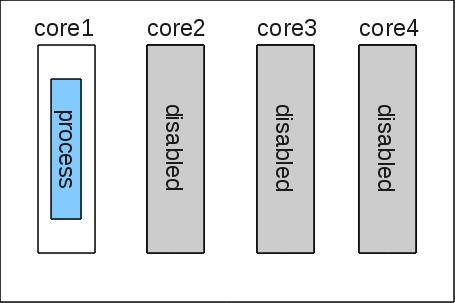
\includegraphics[scale=0.4]{./Figures/disabled_cores.jpg}
    \rule{35em}{0.5pt}
  \caption[Disabled cores]{One core is hosting the MPI process, others are disabled}
  \label{fig:disabled_cores}
\end{figure}
\begin{figure}[htbp]
  \centering
    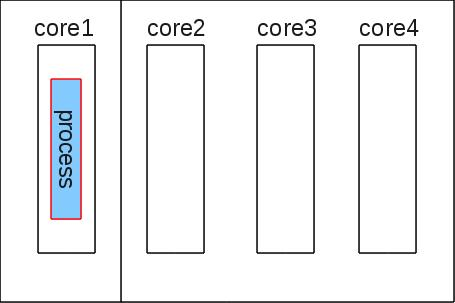
\includegraphics[scale=0.4]{./Figures/bind_to_core.jpg}
    \rule{35em}{0.5pt}
  \caption[Core binding]{None of the cores are disabled, but the
    process is bound to one core, so it doesn't migrate}
  \label{fig:core_binding}
\end{figure}
\subsection{Impact of instrumentation}
In the context of the collection of traces, "instrumenting" an
application means specifying what kind of data we need and which
part of the program we need it from. This can be done either directly
(by inserting function calls or macros that record the data we want),
or by using an overlay library for this purpose. For example, in the
case of TAU, there is a feature called selective instrumentation,
which provides us with the possibility to specify which functions we
want to be traced.\\
When instrumenting the application, it is important to know at what
degree we want to do it. We want to collect the data we need, but the
greater the degree of performance instrumentation in the program, the
higher the likelihood that the performance measurements will alter the
program's performance, an outcome called \emph{performance
 perturbation}.\cite{sm06} In the case of most performance tools, TAU
included, this is a concern that the developers try to address by
reducing the overhead of the performance measurements as much as
possible. It is worth noting though that although the overhead the
measurements cause might be reduced, they can't be completely
eliminated, since the tracing operations have to
be handled by the processor as well. Because of this, the user has to be
very careful when instrumenting an application. There are two main
concerns that come up in our case.
\paragraph{Time overhead}
Instrumentation can have a sizeable negative impact on the performance
of the application. If the instrumentation causes a noticeable
increase in running time, the simulator's prediction might be off,
since it doesn't take into account the instrumentation overhead (as
instrumentation is not part of the experiment).
\paragraph{Impact on hardware counter values}
As mentioned before, when collecting time-independent traces, we use
hardware counters to measure the volume of each operation. The
hardware counter doesn't distinguish between events related to the
experiment and tracing operations, thus all of them are taken into
account. The result is that the collected trace represents the traced
experiment, while we want information from just the experiment,
without the traces. If the difference is too big, this can make our
simulations look inaccurate. The impact it can have when using
off-line simulation, where the simulator replays the traces corrupted
with this overhead is shown in \cite{dms12}.\\[0.5cm]
In \cite{dms12}, the authors propose an instrumentation method as a
correction to their previous work in \cite{dmsq11}. The problem was
that there was a sizeable overhead caused mainly by TAU building the
whole call path of the instrumented application. While it can be
very useful when trying to find bottlenecks in the application, this
information is not needed for simulation purposes. In the proposed
method, we tell TAU to exclude all of the source files from the
instrumentation. This way, instrumentation becomes minimal, while
still covering our specific needs: the hardware counter will be
triggered at each MPI call to measure the number of executed
instructions in the operations. All of the information related to MPI
calls, i.e. the id of the process that made the call, the name of the
function and its parameters are traced. All this while both the time
overhead and the hardware counter value discrepancies are considerably
reduced, as shown in \cite{dms12}.
\subsection{Clock synchronization}
\label{sec:clock_synch}
Another obstacle that comes up when wanting to analyze trace data
generated in a distributed system is related to clock
synchronization. When running a parallel experiment on a distributed
system that uses multiple nodes, all the used nodes produce separate
trace streams independently of each other. The problem is that between
the local processor clocks of different nodes, there almost always exists
some amount of discrepancy, mostly related to the temperature
of the processor. No matter how little this discrepancy is,
it can accumulate over time, as well as it can change the logical
event order, which requires a message to be received only after being
sent from the other node. This is also referred to as the \emph{clock
condition}.\cite{wbswpclg00}\cite{brwl09} Such inaccuracy in the traces
can lead to false conclusions when doing the performance
analysis. Even though in our work we want to use time-independent
traces, violations of the clock condition is still a problem we have
to be able to handle.\\
The problem could be easily avoided if every process would use a
global clock instead of the local clock of the node it's running
on. The problem with this approach is that accessing the global clock
can be much more expensive than accessing the local clock, thus
causing performance issues, as well as it's not available on every
platform. In \cite{wbswpclg00}, the authors use an IBM switch
adapter's globally synchronized clock's register to periodically
collect global clock records for each node, thus being able to correct
the local clock discrepancies after the experiment finished.\\
The main problem with this is, as already mentioned, that although
some systems do offer a relatively
accurate global clock, many other systems are only equipped with
processor-local clocks, in which case the problem has to be approached
from another direction. There exist clock synchronization protocols,
such as NTP \cite{m92}, which provides a widely used solution to align
the clocks to a certain degree by adjusting local clocks at regular
intervals to a globally accessible time server. Unfortunately, due to
varying network latencies, this method still leaves an error rate
of about 1 ms when synchronizing, which is not good enough for our
purposes.
TAU handles this problem with another post-processing approach, using
an extended and parallelized version of the \emph{controlled logical
clock} (CLC) algorithm, which is described in \cite{brwl09}. CLC
retroactively corrects clock condition violations in event traces of
message-passing applications by shifting message events in time. When
making such a correction, CLC makes certain precautions, since
after the modification of individual timestamps, the length of
intervals between events in the immediate vicinity of the affected
event might change, as well as new clock violations might be
introduced.\\[0.5cm]
In this chapter, we talked about the reasoning behind why we need a
trace automation framework. We described certain attributes that we
want our tool to have, as well as the current trace collection method
that we'd like to make easier and more straightforward. We also
depicted some of the obstacles that we need to pay attention to when
collecting traces, such as the problem with multiple cores, the impact
of instrumentation on the performance, or clock synchronization
problems. When discussing these, we also mentioned certain methods to
overcome these problems. In the next
chapter, we'll discuss more specific details about the implementation
of the framework.
